\documentclass[
    xcolor={svgnames,dvipsnames},
    hyperref={colorlinks, citecolor=DeepPink4, linkcolor=DarkRed, urlcolor=DarkBlue}
    ]{beamer}  % for hardcopy add 'trans'


\mode<presentation>
{
  \usetheme{Singapore}
  % or ...
  \setbeamercovered{transparent}
  % or whatever (possibly just delete it)
}

%\usefonttheme{professionalfonts}
%\usepackage[english]{babel}
% or whatever
%\usepackage[latin1]{inputenc}
% or whatever
%\usepackage{times}
%\usepackage[T1]{fontenc}
% Or whatever. Note that the encoding and the font should match. If T1
% does not look nice, try deleting the line with the fontenc.

%\usepackage{fontspec}
%\setmonofont{CMU Typewriter Text}
%\setmonofont{Consolas}

\usepackage{fontspec} 
%\usepackage[xcharter]{newtxmath}
%\setmainfont{XCharter}
\usepackage{unicode-math}
%\setmathfont{XCharter-Math.otf}
\setmonofont{DejaVu Sans Mono}[Scale=MatchLowercase] % provides unicode characters 



%%%%%%%%%%%%%%%%%%%%%% start my preamble %%%%%%%%%%%%%%%%%%%%%%

\addtobeamertemplate{navigation symbols}{}{%
    \usebeamerfont{footline}%
    \usebeamercolor[fg]{footline}%
    \hspace{1em}%
    \insertframenumber/\inserttotalframenumber
}


\usepackage{graphicx}
\usepackage{amsmath, amssymb, amsthm}
\usepackage{bbm}
\usepackage{mathrsfs}
\usepackage{xcolor}
\usepackage{fancyvrb}


% Quotes at start of chapters / sections
\usepackage{epigraph}  
%\renewcommand{\epigraphflush}{flushleft}
%\renewcommand{\sourceflush}{flushleft}
\renewcommand{\epigraphwidth}{6in}

%% Fonts

%\usepackage[T1]{fontenc}
\usepackage{mathpazo}
%\usepackage{fontspec}
%\defaultfontfeatures{Ligatures=TeX}
%\setsansfont[Scale=MatchLowercase]{DejaVu Sans}
%\setmonofont[Scale=MatchLowercase]{DejaVu Sans Mono}
%\setmathfont{Asana Math}
%\setmainfont{Optima}
%\setmathrm{Optima}
%\setboldmathrm[BoldFont={Optima ExtraBlack}]{Optima Bold}

% Some colors

\definecolor{aquamarine}{RGB}{69,139,116}
\definecolor{midnightblue}{RGB}{25,25,112}
\definecolor{darkslategrey}{RGB}{47,79,79}
\definecolor{darkorange4}{RGB}{139,90,0}
\definecolor{dogerblue}{RGB}{24,116,205}
\definecolor{blue2}{RGB}{0,0,238}
\definecolor{bg}{rgb}{0.95,0.95,0.95}
\definecolor{DarkOrange1}{RGB}{255,127,0}
\definecolor{ForestGreen}{RGB}{34,139,34}
\definecolor{DarkRed}{RGB}{139, 0, 0}
\definecolor{DarkBlue}{RGB}{0, 0, 139}
\definecolor{Blue}{RGB}{0, 0, 255}
\definecolor{Brown}{RGB}{165,42,42}


\setlength{\parskip}{1.5ex plus0.5ex minus0.5ex}

%\renewcommand{\baselinestretch}{1.05}
%\setlength{\parskip}{1.5ex plus0.5ex minus0.5ex}
%\setlength{\parindent}{0pt}

% Typesetting code
\definecolor{bg}{rgb}{0.95,0.95,0.95}
\usepackage{minted}
\setminted{mathescape, frame=lines, framesep=3mm}
\usemintedstyle{friendly}
%\newminted{python}{}
%\newminted{c}{mathescape,frame=lines,framesep=4mm,bgcolor=bg}
%\newminted{java}{mathescape,frame=lines,framesep=4mm,bgcolor=bg}
%\newminted{julia}{mathescape,frame=lines,framesep=4mm,bgcolor=bg}
%\newminted{ipython}{mathescape,frame=lines,framesep=4mm,bgcolor=bg}


\newcommand{\Fact}{\textcolor{Brown}{\bf Fact. }}
\newcommand{\Facts}{\textcolor{Brown}{\bf Facts }}
\newcommand{\keya}{\textcolor{turquois4}{\bf Key Idea. }}
\newcommand{\Factnodot}{\textcolor{Brown}{\bf Fact }}
\newcommand{\Eg}{\textcolor{ForestGreen}{Example. }}
\newcommand{\Egs}{\textcolor{ForestGreen}{Examples. }}
\newcommand{\Ex}{{\bf Ex. }}



\renewcommand{\theFancyVerbLine}{\sffamily
    \textcolor[rgb]{0.5,0.5,1.0}{\scriptsize {\arabic{FancyVerbLine}}}}

\newcommand{\navy}[1]{\textcolor{Blue}{\bf #1}}
\newcommand{\brown}[1]{\textcolor{Brown}{\sf #1}}
\newcommand{\green}[1]{\textcolor{ForestGreen}{\sf #1}}
\newcommand{\blue}[1]{\textcolor{Blue}{\sf #1}}
\newcommand{\navymth}[1]{\textcolor{Blue}{#1}}
\newcommand{\emp}[1]{\textcolor{DarkOrange1}{\bf #1}}
\newcommand{\red}[1]{\textcolor{Red}{\bf #1}}

% Symbols, redefines, etc.

\newcommand{\code}[1]{\texttt{#1}}

\newcommand{\argmax}{\operatornamewithlimits{argmax}}
\newcommand{\argmin}{\operatornamewithlimits{argmin}}

\DeclareMathOperator{\cl}{cl}
\DeclareMathOperator{\interior}{int}
\DeclareMathOperator{\Prob}{Prob}
\DeclareMathOperator{\determinant}{det}
\DeclareMathOperator{\trace}{trace}
\DeclareMathOperator{\Span}{span}
\DeclareMathOperator{\rank}{rank}
\DeclareMathOperator{\cov}{cov}
\DeclareMathOperator{\corr}{corr}
\DeclareMathOperator{\var}{var}
\DeclareMathOperator{\mse}{mse}
\DeclareMathOperator{\se}{se}
\DeclareMathOperator{\row}{row}
\DeclareMathOperator{\col}{col}
\DeclareMathOperator{\range}{rng}
\DeclareMathOperator{\dimension}{dim}
\DeclareMathOperator{\bias}{bias}


% mics short cuts and symbols
\newcommand{\st}{\ensuremath{\ \mathrm{s.t.}\ }}
\newcommand{\setntn}[2]{ \{ #1 : #2 \} }
\newcommand{\cf}[1]{ \lstinline|#1| }
\newcommand{\fore}{\therefore \quad}
\newcommand{\tod}{\stackrel { d } {\to} }
\newcommand{\toprob}{\stackrel { p } {\to} }
\newcommand{\toms}{\stackrel { ms } {\to} }
\newcommand{\eqdist}{\stackrel {\textrm{ \scriptsize{d} }} {=} }
\newcommand{\iidsim}{\stackrel {\textrm{ {\sc iid }}} {\sim} }
\newcommand{\1}{\mathbbm 1}
\newcommand{\dee}{\,{\rm d}}
\newcommand{\given}{\, | \,}
\newcommand{\la}{\langle}
\newcommand{\ra}{\rangle}

\newcommand{\boldA}{\mathbf A}
\newcommand{\boldB}{\mathbf B}
\newcommand{\boldC}{\mathbf C}
\newcommand{\boldD}{\mathbf D}
\newcommand{\boldM}{\mathbf M}
\newcommand{\boldP}{\mathbf P}
\newcommand{\boldQ}{\mathbf Q}
\newcommand{\boldI}{\mathbf I}
\newcommand{\boldX}{\mathbf X}
\newcommand{\boldY}{\mathbf Y}
\newcommand{\boldZ}{\mathbf Z}

\newcommand{\bSigmaX}{ {\boldsymbol \Sigma_{\hboldbeta}} }
\newcommand{\hbSigmaX}{ \mathbf{\hat \Sigma_{\hboldbeta}} }

\newcommand{\RR}{\mathbbm R}
\newcommand{\NN}{\mathbbm N}
\newcommand{\PP}{\mathbbm P}
\newcommand{\EE}{\mathbbm E \,}
\newcommand{\XX}{\mathbbm X}
\newcommand{\ZZ}{\mathbbm Z}
\newcommand{\QQ}{\mathbbm Q}

\newcommand{\fF}{\mathcal F}
\newcommand{\dD}{\mathcal D}
\newcommand{\lL}{\mathcal L}
\newcommand{\gG}{\mathcal G}
\newcommand{\hH}{\mathcal H}
\newcommand{\nN}{\mathcal N}
\newcommand{\pP}{\mathcal P}




\title{Python and the AI Revolution}


\author{Chase Coleman and John Stachurski}


\date{March 2024}


\begin{document}

\begin{frame}
  \titlepage
\end{frame}







\begin{frame}
    \frametitle{Topics}

    We will discuss

    \begin{itemize}
        \item AI-driven scientific computing
        \vspace{0.5em}
        \item Where are we heading?
        \vspace{0.5em}
        \item Economic applications?
    \end{itemize}

        \vspace{0.5em}
        \vspace{0.5em}
    Sides

    \url{https://github.com/QuantEcon/imf_2024}

\end{frame}



\begin{frame}
    \frametitle{AI-driven scientific computing}

    Key players
    %
    \begin{itemize}
        \item OpenAI (ChatGPT, Whisper), Microsoft 
        \vspace{0.5em}
        \item Google Research, Google DeepMind
        \vspace{0.5em}
        \item Meta
        \vspace{0.5em}
        \item Anthropic, etc.
    \end{itemize}

    Platforms / libraries

    \begin{itemize}
        \item PyTorch (OpenAI, Meta's LLaMA 2,  Stable Diffusion)
        \vspace{0.5em}
        \item Google JAX (Google's Gemini)
        \vspace{0.5em}
        \item Tensorflow, Keras, Mojo?
    \end{itemize}
    
\end{frame}


\begin{frame}
    \frametitle{Lightening introduction to deep learning}
    
    Supervised deep learning: find a good approximation to an unknown functional
    relationship
    %
    \begin{equation*}
        y = f(x)
    \end{equation*}

    \begin{itemize}
        \item $x$ is the input and $y$ is the output
    \end{itemize}

        \vspace{0.5em}
        \vspace{0.5em}
        \vspace{0.5em}
    \Egs
    %
    \begin{itemize}
        \item $x = $ unfinished sentence, $y = $ next word
        \vspace{0.5em}
        \item $x = $ weather sensor data, $y = $ max temp tomorrow
    \end{itemize}

\end{frame}


\begin{frame}
    \frametitle{Training}

    Nonlinear regression: Take data set $(x_i, y_i)_{i=1}^n$ and solve
    %
    \begin{equation*}
        \min_\theta  \ell(\theta) = \sum_{i=1}^n (y_i - f_\theta(x_i))^2
        \quad \st \quad \theta \in \Theta
    \end{equation*}

    \vspace{0.5em}
    In the case of ANNs, we consider all $f_\theta$ having the form
    %
    \begin{equation*}
        f_\theta
        = \sigma \circ A_{1} \circ \cdots \circ \sigma \circ A_{k} 
    \end{equation*}
    %
    where
    %
    \begin{itemize}
        \item $A_{i} x = W_{i} x + b_{i} $ is an affine map 
        \vspace{0.5em}
        \item $\sigma$ is a nonlinear ``activation'' function
    \end{itemize}

\end{frame}


\begin{frame}
    

    Minimizing a smooth loss functions
    
    \begin{figure}
       \begin{center}
        \scalebox{0.15}{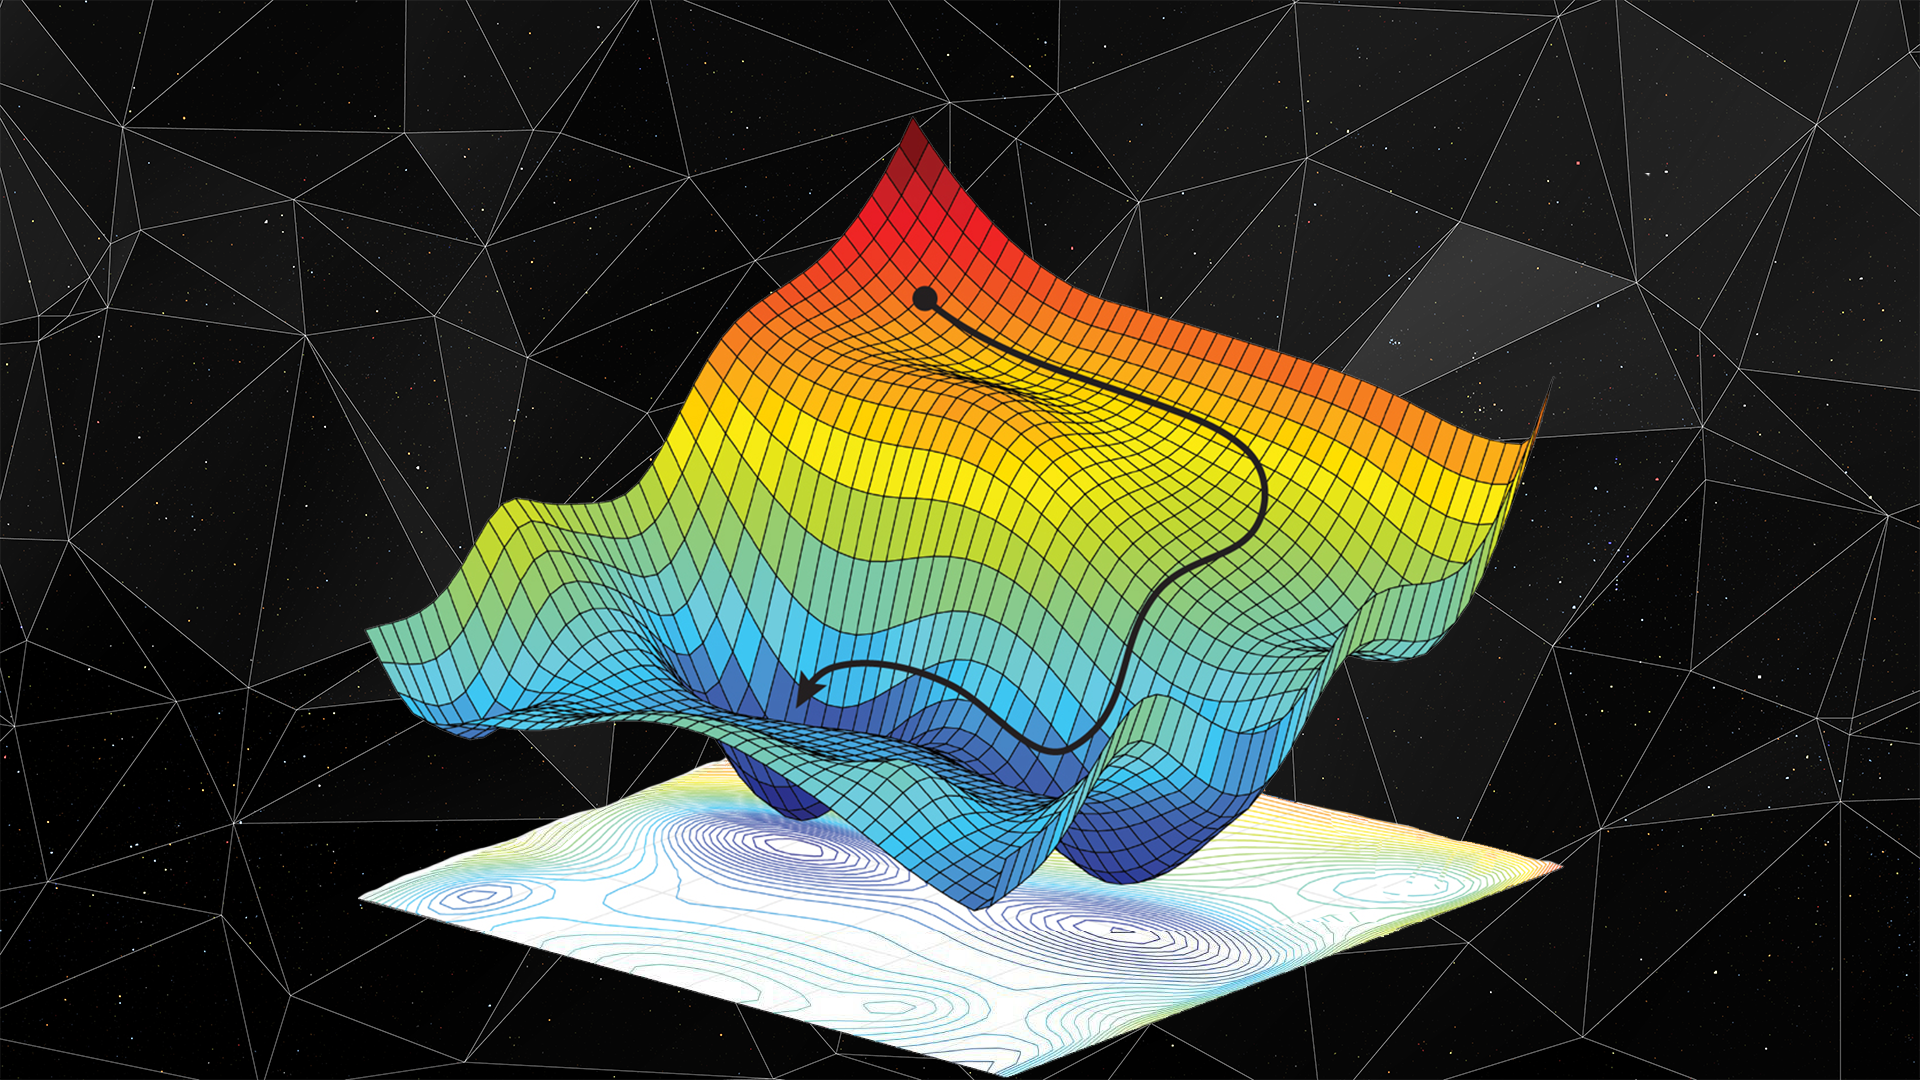
\includegraphics[trim={0cm 0cm 0cm 0cm},clip]{gdi.png}}
       \end{center}
    \end{figure}

    Source: \url{https://danielkhv.com/}

\end{frame}


\begin{frame}
    
    \begin{figure}
       \begin{center}
        \scalebox{0.18}{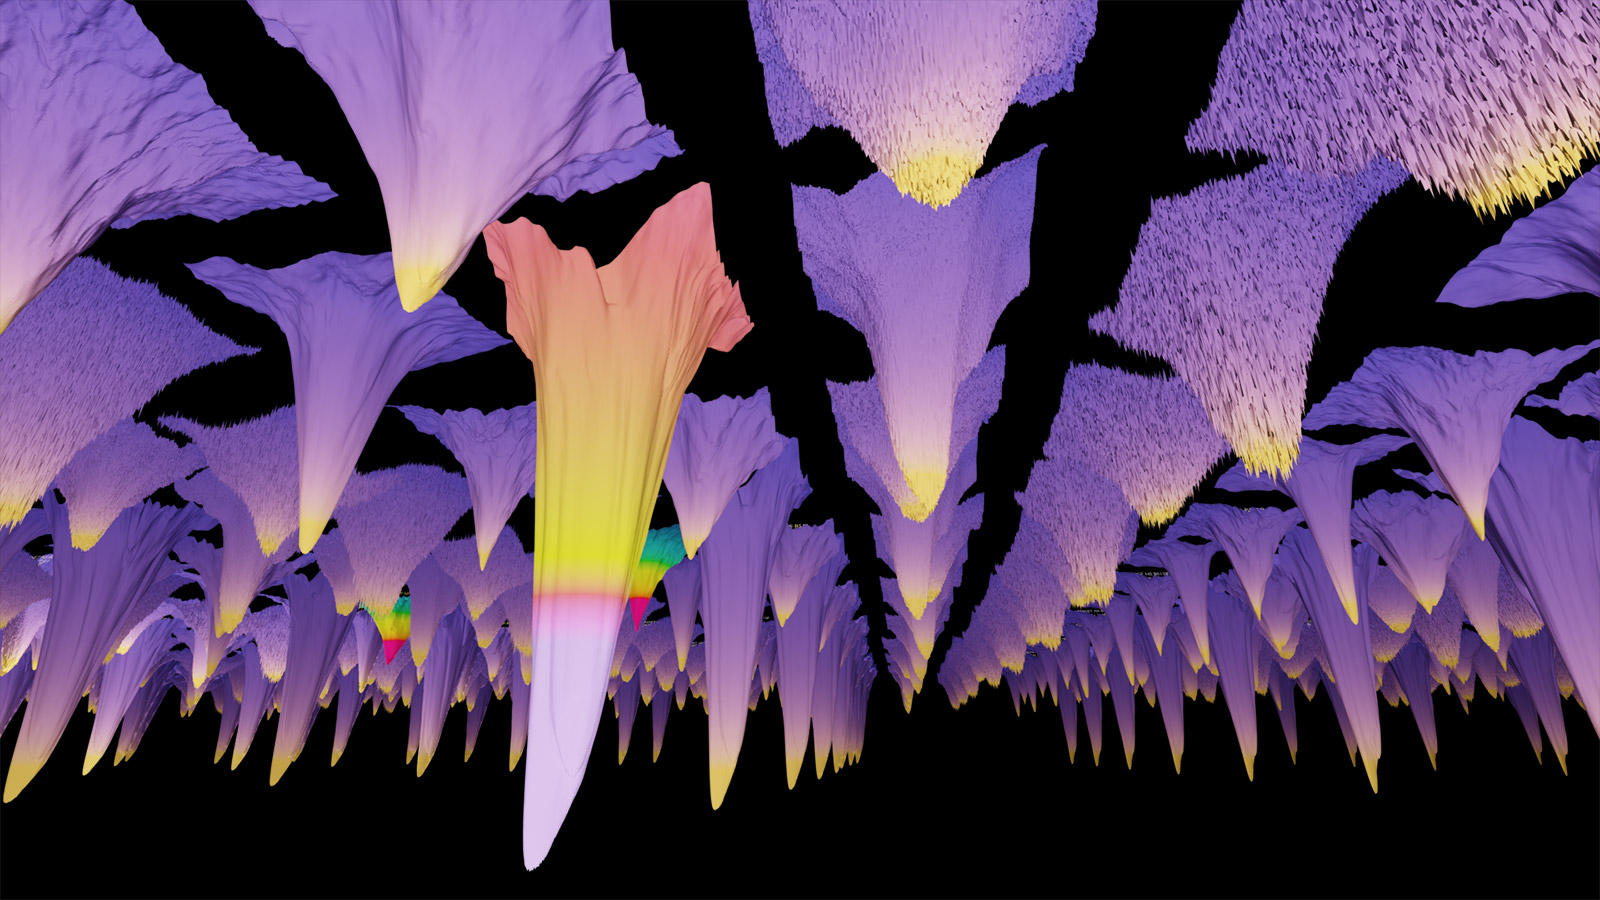
\includegraphics[trim={0cm 0cm 0cm 0cm},clip]{loss2.jpg}}
       \end{center}
    \end{figure}

    Source: \url{https://losslandscape.com/gallery/}

\end{frame}

\begin{frame}
    

    Core elements
    %
    \begin{itemize}
        \item automatic differentiation!
        \vspace{0.5em}
        \item parallelization (CPUs / GPUs / TPUs)!
        \vspace{0.5em}
        \item Compilers / JIT-compilers!
    \end{itemize}

\end{frame}


\begin{frame}[fragile]
    
    \begin{minted}{python}
import jax.numpy as jnp
from jax import grad, jit

def predict(params, x):
  for W, b in params:
    y = jnp.dot(W, x) + b
    x = jnp.tanh(y)  
  return y                

def loss(params, x, targets):
  preds = predict(params, x)
  return jnp.sum((preds - targets)**2)

grad_loss = jit(grad(loss))  
# Now use gradient descent on the loss function
    \end{minted}

\end{frame}




\begin{frame}

    
    ``ECMWF's weather forecasting model is considered the gold standard for
        medium-term weather forecasting\ldots 
        Google DeepMind claims
        in an non-peer-reviewed paper to have beat it 90\% of the time\ldots''

    \vspace{0.5em}
    \vspace{0.5em}

    ``Traditional forecasting models are big, complex computer algorithms based
    on atmospheric physics and take hours to run. AI models can create forecasts
    in just seconds.'' 
    \vspace{0.5em}
    \vspace{0.5em}

    $\quad \qquad$$\quad \qquad$ Source: MIT Technology Review  

\end{frame}


\begin{frame}
    

    Relevant to economics?

    \vspace{0.5em}

    \begin{itemize}
        \item Deep learning provides massively powerful pattern recognition
            systems
        \vspace{0.5em}
        \item But macroeconomic data is far more limited than weather
            observation sensor data\ldots
        \vspace{0.5em}
        \item and generally nonstationary
        \vspace{0.5em}
        \item and laws of motion change with policies (Lucas critique)
    \end{itemize}

    \vspace{0.5em}

    Possible applications:

    \begin{itemize}
        \item Finding stylized facts? Testing causal relationships?
        \vspace{0.5em}
        \item Numerical methods -- approximating high-dimensional functions
    \end{itemize}

\end{frame}


\begin{frame}
    
    One point of view

    \begin{itemize}
        \item Deep learning is not very relevant for policy-centric macroeconomic modeling
        \vspace{0.5em}
        \item Deep learning is yet to prove itself as a ``better'' approach to
            numerical methods
        \vspace{0.5em}
        \item And yet, at the same time, the AI computing revolution is
            generating tools that are enormously beneficial for macroeconomic
            modeling
        \vspace{0.5em}
            \begin{itemize}
                \item autodiff, JIT compilers, parallelization, GPUs, etc.
            \end{itemize}
        \vspace{0.5em}
        \item We can take full advantage of them right now\ldots
    \end{itemize}

\end{frame}

\end{document}


